% -*- coding: utf-8; -*-

\chapter{Fundamentação Teórica}

O desenvolvimento de campos de petróleo ocorre sob condições de incerteza associadas à caracterização geológica do reservatório, bem como a parâmetros econômicos e tecnológicos. Essas incertezas influenciam diretamente o valor do projeto. O baixo desempenho de algumas empresas de petróleo é consequência do reduzido investimento aplicado em ferramentas de suporte à decisão e da ausência de investimentos suficientes para estimar corretamente o retorno do projeto, o que pode levar tanto à superestimação dos ganhos quanto à subestimação das perdas.

Três tipos de riscos no desenvolvimento de campos de petróleo devem ser considerados no processo de tomada de decisão:
\begin{enumerate}
    \item \textbf{perda de oportunidade}: um prospecto é considerado não econômico e abandonado, quando na verdade seria viável economicamente;
    \item \textbf{desenvolvimento não econômico}: um campo inviável é desenvolvido por ter sido erroneamente considerado econômico;
    \item \textbf{desenvolvimento subótimo}: um campo é desenvolvido, mas gera retorno inferior ao máximo possível, que poderia ser obtido se o modelo de reservatório correto tivesse sido considerado.
\end{enumerate}

O risco envolvido na fase de desenvolvimento pode ser reduzido se informações adicionais forem obtidas para diminuir ou até eliminar uma determinada incerteza. Entretanto, a aquisição de informação está diretamente associada a custos. Por isso, antes de decidir pela obtenção de informação,  sugere analisar dois aspectos: se vale a pena adquirir informação adicional e se tal informação é de fato capaz de melhorar o processo decisório. Uma ferramenta consistente que pode ser utilizada como critério no processo de decisão é o \textit{Valor da Informação (VOI)}, que combina incertezas do reservatório com suas potenciais consequências econômicas. 


\section{Valor da Informação}

A prática profissional em engenharia de petróleo e geociências está fortemente associada à aquisição de informações, obtidas sob diversas formas e em múltiplos contextos. O termo \textbf{informação} é usado aqui em um sentido amplo, incluindo coleta de dados, realização de estudos técnicos, contratação de consultores, execução de testes diagnósticos, etc. A expectativa é que a redução da incerteza aumente a chance de que nossas decisões resultem no desfecho desejado. De fato, a única outra razão válida para coletar informação ou realizar análises técnicas é o cumprimento de exigências regulatórias.

A questão fundamental em qualquer processo de coleta de informação é se a redução esperada da incerteza compensa o custo de se obter a informação. A técnica de \textit{Value of Information} (VOI), em português Valor da Informação, é projetada justamente para responder a essa questão \cite{01}.

\subsection{Princípios da Aquisição de Informação}

O objetivo de um cálculo de VOI é estimar o valor de um exercício proposto de coleta de informações, de modo que a decisão de implementá-lo ou não seja feita em bases econômicas. Para que a informação seja valiosa, deve existir uma dependência probabilística entre a informação e os resultados do evento incerto de interesse (relevância). Além disso, o evento de interesse deve impactar suficientemente uma métrica de decisão a ponto de podermos alterar nossa decisão (materialidade). Finalmente, seu valor deve exceder o seu custo, caso em que a regra implícita de investimento recomenda adquirir a informação (valor maior que o custo). O custo de aquisição da informação depende da natureza da informação. O cálculo dos custos inclui salários da equipe, custos de oportunidade e custos diretos óbvios.  

O VOI pode ser entendido como o valor atribuído às probabilidades atualizadas. Para calcular esse valor, são necessárias as seguintes informações:  

\begin{enumerate}
    \item \textbf{Probabilidade atuais}, ou \textit{a priori}, dos possíveis resultados que a variável pode assumir (por exemplo, 30\% de chance de o fator de recuperação ser baixo e 70\% de chance de ser alto).  
    \item \textbf{Estimativas de confiabilidade (verossimilhança)} da eficácia da informação em predizer os resultados (por exemplo, quando o fator de recuperação é conhecido como alto, estudos de simulação de reservatórios 3D indicam corretamente ``alto'' em 80\% dos casos).  
    \item \textbf{Valores de projeto em termos monetários} para cada uma das possíveis combinações de resultados (por exemplo, VPL de +600 milhões de USD se o fator de recuperação for alto e  -100 milhões de USD se for baixo).  
\end{enumerate}

Embora os valores de projeto possam ser derivados por meio de análise determinística, recomenda-se o uso do Valor Presente Líquido (VPL, do inglês \textit{Net Present Value -- NPV}) esperado, obtido via simulação de Monte Carlo de outras incertezas, devido às complexas inter-relações frequentemente envolvidas.


\subsection{Valor Esperado da Informação}

O cálculo do VOI costuma ser representado em árvores de decisão, pois elas trazem clareza ao processo. O procedimento envolve comparar duas árvores:  

\begin{itemize}
    \item A primeira árvore representa o valor esperado do projeto com as probabilidades atuais.  
    \item A segunda árvore representa o valor esperado do projeto com as probabilidades atualizadas, resultantes da aquisição da informação.  
\end{itemize}

A diferença entre os dois valores fornece o \textbf{VOI esperado}. Utilizamos o termo \textbf{esperado} em seu sentido matemático estrito — o valor obtido ao aplicar repetidamente a metodologia do VoI em diversas decisões. Antes de detalhar o procedimento de cálculo, consideremos primeiro alguns limites intuitivos do VoI:

\begin{itemize}
    \item \textbf{Limite inferior}: Se a informação não altera a decisão, seu valor esperado é zero, independentemente do custo.  
    \item \textbf{Limite superior}: A informação perfeita (sem erro) fornece o valor máximo possível, denominado \textit{Valor Esperado da Informação Perfeita} (EVPI). Este limite superior serve como referência: nenhum processo de aquisição de informação pode exceder o EVPI.  
\end{itemize}

O cálculo do EVPI não depende da existência de métodos perfeitos de aquisição de informação, mas sim de fornecer um \textit{benchmark} para avaliar qualquer processo de coleta de informação. Se o custo do processo excede o EVPI, não há motivo para prosseguir com a proposta. Se o EVPI indicar que vale a pena avançar, procede-se ao cálculo do valor esperado da informação imperfeita (EVII), que leva em conta a confiabilidade da informação obtida.

\subsection{Etapas no Cálculo do VOI}

Os principais procedimentos para conduzir um estudo de VOI são descritos a seguir. Posteriormente, estes passos serão ilustrados por meio de uma decisão simplificada.

\begin{enumerate}
    \item Calcular o valor esperado da decisão a ser tomada no estado atual (isto é, sem a informação). Este cálculo é denominado \textbf{valor do projeto base}.
    \item Formular a estrutura da situação de decisão de modo a incluir a nova informação. Isso é feito adicionando um novo ramo ao primeiro nó da árvore de decisão para representar a escolha de adquirir informação. Este ramo leva a um nó de incerteza, cujo evento incerto corresponde aos resultados do exercício de coleta de informação.
    \item Calcular o valor da informação perfeita. Se o EVPI for insignificante ou menor que o custo de aquisição da informação, não se deve coletar a informação e deve-se escolher a alternativa de maior valor no projeto base. Caso contrário, prosseguir para o Passo 4.    
    \item Calcular o valor do projeto com a informação real, ou imperfeita. Este passo é subdividido em:
    \begin{enumerate}
        \item Estimar as probabilidades de verossimilhança, isto é, $P(\text{informação diz} \mid \text{mundo real é})$.
        \item Calcular as probabilidades atualizadas (posteriores) pelo Teorema de Bayes.
        \item Inserir as probabilidades atualizadas na árvore de decisão e resolver para obter o valor do projeto.
    \end{enumerate}
    \item Calcular o EVII, obtido pela diferença entre os valores dos Passos 4 e 1. Comparar essa diferença com o custo de aquisição da informação.
    \item Realizar uma análise de sensibilidade para verificar a robustez da decisão diante de variações nas probabilidades e nos \textit{payoffs}. 
\end{enumerate}

A parte mais complexa do procedimento anterior é o Passo 2 --- garantir que a formulação da situação de decisão inclua a informação antecipada. Para ilustrar, considere o seguinte exemplo simplificado. Suponha uma decisão binária: realizar uma ação (por exemplo, perfurar um poço) ou não. Denotamos essas alternativas como $D_{1}$ e $D_{2}$, ver Figura~\ref{fig:2.1}.  

\begin{figure} [h]
  \begin{center}
    \includegraphics[height=220pt,width=380pt]{images/generic_VOI.png}
    \caption{Árvore de decisão genérica do VoI. Fonte: \cite{01}.}\label{fig:2.1}
  \end{center}
\end{figure}

Há um evento incerto $B$ com dois possíveis resultados: $B_{1}$ e $B_{2}$ (por exemplo, o poço é comercial ou não). As probabilidades desses resultados são $P(B_{1})$ e $P(B_{2})$. Se escolhermos $D_{1}$, o valor do projeto é $NPV(B_{1})$ ou $NPV(B_{2})$, dependendo do resultado. Se escolhermos $D_{2}$, assumimos payoff igual a USD 0. Esse caso constitui o \textit{projeto base} (Passo 1). Para incluir a opção de coletar informação adicional, adicionamos uma terceira alternativa $D_{A}$ ao nó inicial da árvore, indicando a decisão de adquirir informação, $A$. Os possíveis resultados dessa informação, $A_{1}$ ou $A_{2}$, são conhecidos por serem dependentes dos resultados de interesse, $B_{1}$ e $B_{2}$. Um exemplo seria um levantamento sísmico 3D, cujos resultados podem ser “Bright Spot” ($A_{1}$) ou “No Bright Spot” ($A_{2}$). Nesse ponto, não conhecemos as probabilidades de $A_{1}$ ou $A_{2}$, mas uma vez conhecidas, retomamos a decisão original. O problema de decisão é então modelado replicando a árvore do projeto base em cada ramo correspondente a $A_{1}$ e $A_{2}$. As probabilidades de $B$, por estarem relacionadas às probabilidades de $A$, são indicadas como probabilidades condicionais. Por exemplo, se o levantamento sísmico ($A_{1}$) indicar “Bright Spot” e decidirmos executar o projeto $D_{1}$, o poço poderá ser comercial com probabilidade $P(\text{Comercial} \mid A_{1})$ ou não comercial com probabilidade $P(\text{Não Comercial} \mid A_{1})$. Dessa forma, a situação de decisão passa a incluir a opção de coletar informação. O próximo passo é calcular as probabilidades necessárias e resolver a árvore normalmente. Supondo que tenhamos dados de confiabilidade sobre a eficácia de “Bright Spots” na previsão de poços comerciais, podemos combiná-los com as probabilidades a priori por meio do processo de \textit{tree-flipping} (inversão da árvore de decisão) que permite combinar probabilidades a priori com informações de confiabilidade, conforme ilustrado na Figura~\ref{fig:2.2}.  

\begin{figure} [h]
  \begin{center}
    \includegraphics[height=220pt,width=380pt]{images/tree_flipping.png}
    \caption{Inversão da árvore de decisão. Fonte: \cite{01}.}\label{fig:2.2}
  \end{center}
\end{figure}

A soma das probabilidades dos possíveis resultados da aquisição de informação, $P(A_{1})$ e $P(A_{2})$, corresponde à probabilidade total. Esse é justamente o denominador do \textbf{Teorema de Bayes}, que pode ser escrito de forma geral como:

\begin{equation}
P(B_{i} \mid A) = \frac{P(A \mid B_{i}) \, P(B_{i})}{\sum_{j=1}^{n} P(A \mid B_{j}) \, P(B_{j})}.
\end{equation}
\par\medskip % força fim de parágrafo + espaço
No caso específico do exemplo acima, obtemos as seguintes probabilidades atualizadas:
\begin{align}
P(B_{1} \mid A_{1}) &= \frac{P(A_{1}\mid B_{1}) P(B_{1})}{P(A_{1}\mid B_{1}) P(B_{1}) + P(A_{1}\mid B_{2}) P(B_{2})} \\[6pt]
P(B_{2} \mid A_{1}) &= \frac{P(A_{1}\mid B_{2}) P(B_{2})}{P(A_{1}\mid B_{1}) P(B_{1}) + P(A_{1}\mid B_{2}) P(B_{2})} \\[6pt]
P(B_{1} \mid A_{2}) &= \frac{P(A_{2}\mid B_{1}) P(B_{1})}{P(A_{2}\mid B_{1}) P(B_{1}) + P(A_{2}\mid B_{2}) P(B_{2})} \\[6pt]
P(B_{2} \mid A_{2}) &= \frac{P(A_{2}\mid B_{2}) P(B_{2})}{P(A_{2}\mid B_{1}) P(B_{1}) + P(A_{2}\mid B_{2}) P(B_{2})}
\end{align}

Uma questão central na análise de VoI é a origem das probabilidades a priori e de verossimilhança. Em geral, tais probabilidades derivam de \textit{avaliações subjetivas}, baseadas no conhecimento dos especialistas sobre a situação ou dados disponíveis. A subjetividade é inerente à análise de decisão: os modelos são aproximações da realidade e frequentemente dependem de julgamentos sem dados empíricos diretos.

\textbf{Priors:} As distribuições a priori descrevem o estado de conhecimento sobre o evento incerto antes da obtenção de novas informações. Essa interpretação como "grau de crença" é amplamente aceita e permite o uso de qualquer fonte de conhecimento ou experiência relevante. Ser capaz de avaliar corretamente distribuições a priori é uma habilidade essencial para engenheiros e geocientistas.

\textbf{Likelihood:} A função de verossimilhança representa a probabilidade condicional da informação observada, dado o evento de interesse. Na prática, pode estar relacionada à qualidade ou à confiabilidade da informação adquirida (por exemplo, sísmica, perfis, testes de pressão). A construção da verossimilhança envolve considerar tanto a acurácia dos dados quanto o viés de interpretação. Quando disponíveis, dados históricos podem apoiar a estimação dessas probabilidades, embora sejam raramente formalizados. Em muitos casos, utilizam-se bandas de confiabilidade e análises de sensibilidade para avaliar a robustez das decisões.

Quatro critérios principais determinam se a aquisição de informação é valiosa em um estudo de VoI (\cite{02}, \cite{03}):

\begin{itemize}
    \item \textbf{Observável:} Os resultados da coleta de informação devem ser conhecidos antes da decisão.
    \item \textbf{Relevante:} A informação deve ter o potencial de alterar as crenças sobre a incerteza associada ao problema.
    \item \textbf{Material:} A informação deve ser capaz de modificar a decisão final.
    \item \textbf{Econômica:} O valor esperado da informação deve exceder o custo de adquiri-la.
\end{itemize}

O método de VoI garante que esses critérios sejam satisfeitos e pode ser aplicado a decisões de qualquer complexidade. Entretanto, modelos mais sofisticados podem ser necessários quando múltiplas incertezas ou distribuições contínuas estão envolvidas.

\subsection{Cálculo do Valor da Informação}

O VOI é definido como o valor máximo que o tomador de decisão deveria pagar por informação adicional relevante. Sob a hipótese de neutralidade ao risco, o VOI é dado por \cite{03}:
\begin{equation}
VOI = \mathbb{E}[\text{valor com informação}] - \mathbb{E}[\text{valor sem informação}].
\end{equation}

Se a informação adicional for perfeita, essa quantidade é denominada \textit{Valor da Informação Perfeita} (VOPI) que representa o limite superior de qualquer atividade de coleta de informação. Conforme a terminologia usada na subseção 2.1.2 temos EVPI (Valor Esperado da Informação Perfeita) ou EVII (Valor Esperado da Informação Imperfeita). O valor esperado com informação só pode ser maior do que o valor sem informação se a decisão puder ser alterada em função da informação revelada. Caso o tomador de decisão adote a mesma ação independentemente do resultado do teste, então $VOI = 0$, tornando a coleta de informação inútil para o problema decisório.

Um problema interessante na análise do VOI é o \textbf{problema TALL-N} (\textit{Two-Action Linear-Loss with Normal priors}) que considera um tomador de decisão diante de duas alternativas:
\begin{itemize}
    \item $a_{0}$: alternativa segura, com payoff constante $v$;
    \item $a_{1}$: alternativa arriscada, com payoff incerto descrito por uma variável aleatória $\tilde{x}$ com média $\mu$ e desvio-padrão $\sigma$.
\end{itemize}

Se $\mu < v$, o decisor escolhe $a_{0}$; se $\mu \geq v$, escolhe $a_{1}$; e se $\mu = v$, encontra-se indiferente. 
O valor esperado sem informação adicional é dado por:
\begin{equation}
\mathbb{E}[\text{valor sem informação}] = \max(v, \mu).
\end{equation}

A Figura~\ref{fig:2.3} ilustra o problema TALL-N, em que $\tilde{x}$ é assumida como normalmente distribuída. A padronização $z = \frac{x-\mu}{\sigma}$ permite definir o coeficiente de divergência:
\begin{equation}
c = \frac{\mu - v}{\sigma},
\label{eq:2-8}
\end{equation}
o qual representa a distância entre as duas alternativas em unidades de desvio-padrão.

\begin{figure} [h]
  \begin{center}
    \includegraphics[height=130pt,width=360pt]{images/tall_problem.png}
    \caption{Problema TALL-N com preferência inicial de risco. Fonte: \cite{04}.}\label{fig:2.3}
  \end{center}
\end{figure}

A \textbf{informação perfeita} permite ao decisor sempre escolher a melhor alternativa conforme o verdadeiro estado da natureza. 
Assim, o EVPI é definido por:
\begin{equation}
EVPI = E[\max(v, \tilde{x})] - \max(v, \mu).
\end{equation}

No caso normal (TALL-N), obtém-se a seguinte forma fechada \cite{04}:
\begin{equation}
EVPI =
\begin{cases}
\sigma \, [\phi(c) - c \, \Phi(-c)], & \mu \geq v, \\[6pt]
\sigma \, [\phi(c) + c \, \Phi(c)], & \mu < v,
\end{cases}
\label{eq:2-10}
\end{equation}
em que $\phi(\cdot)$ é a densidade da normal padrão e $\Phi(\cdot)$ sua função de distribuição acumulada.

Quando a \textbf{informação é imperfeita}, mas correlacionada com o payoff incerto, utilizamos o EVII. Considere um sistema de informação $\Theta_{\eta}$, cujo sinal $\theta$ é normalmente distribuído e correlacionado com $\tilde{x}$ por um coeficiente de correlação $\eta > 0$. 
Nesse caso, a média condicional é dada por $E[\tilde{x} \mid \theta] = \mu + \eta \sigma \theta$. Portanto, o EVII é definido por:

\begin{equation}
EVII = E[\max(v, E[\tilde{x} \mid \theta])] - \max(v, \mu),
\label{eq:2-11}
\end{equation}
e pode ser escrito na forma fechada como \cite{04}:
\begin{equation}
EVII =
\begin{cases}
\eta \sigma \, [\phi(\eta^{-1}c) - \eta^{-1}c \, \Phi(-\eta^{-1}c)], & \mu \geq v, \\[6pt]
\eta \sigma \, [\phi(\eta^{-1}c) + \eta^{-1}c \, \Phi(\eta^{-1}c)], & \mu < v.
\end{cases}
\label{eq:2-12}
\end{equation}

Quando a correlação é perfeita ($\eta=1$), temos o caso de informação perfeita, cujos resultados são equivalentes ao EVPI. Por outro lado, a informação imperfeita, com correlação $\eta$, pode ser interpretada como equivalente ao valor da informação perfeita, mas com um desvio-padrão ajustado $\sigma_{\text{ajustado}} = \eta \sigma$, ou seja:
\begin{equation}
    \eta^{-1}c = \frac{\mu - v}{\eta \sigma}
    \label{eq:2-13}
\end{equation}
comparar com a Equação \eqref{eq:2-8}. Isso significa que a qualidade da informação imperfeita pode ser vista como se fosse informação perfeita, porém mais ``difusa'', já que a incerteza é reduzida proporcionalmente a $\eta$.

O EVII é sempre limitado superiormente pelo EVPI, aproximando-se dele quando $\eta \to 1$ e tendendo a zero quando $\eta \to 0$. No limite, quando $c \to \infty$, obtém-se \cite{04}:
\begin{equation}
\lim_{c \to \infty} RVOI^{*}_{\eta} = \eta^2,
\label{eq:2-14}
\end{equation}
onde o sobrescrito $^{*}$ indica que este é o valor máximo do RVOI para um determinado $c$. Assim, define-se o \textit{Relative Value of Information} (RVOI) como a razão entre EVII e EVPI:
\begin{equation}
RVOI_{\eta}^{*} = \frac{EVII}{EVPI} = \eta^2.
\label{eq:2-15}
\end{equation}

Portanto, o RVOI expressa diretamente a fração do valor da informação imperfeita em relação ao valor da informação perfeita, sendo determinado pelo quadrado do coeficiente de correlação, isto é, \(\eta^{2}\) \cite{04}. Na referência \cite{05} temos também a demonstração que $RVOI=\eta^2$ no contexto de perda quadrática e função de regressão linear.

Dado um valor específico de $c$, o RVOI atinge seu valor máximo quando $c = \frac{\sigma}{2R}$, onde $R$ representa a \textit{risk tolerance} do tomador de decisão e $\sigma$ o desvio-padrão.  Nessa condição, a informação imperfeita possui o maior valor relativo em comparação com a informação perfeita, correspondendo ao caso em que o tomador de decisão está indiferente. Assim, o valor máximo do RVOI é expresso por:
\begin{equation}
RVOI_{\eta}^{*} = \frac{\ln \big[2\Phi(-\eta c)\big]}{\ln \big[2\Phi(-c)\big]},
\label{eq:2-16}
\end{equation}

Na Figura~\ref{fig:2.4} é apresentado o gráfico do valor máximo de RVOI* em função do coeficiente de divergência $c$. Observa-se que, para diferentes valores do coeficiente de correlação $\eta$, o comportamento de RVOI* evidencia a importância relativa da informação imperfeita em comparação à informação perfeita. Além disso, a figura permite analisar os valores-limite que fornecem interpretações intuitivas sobre o valor da informação em diferentes cenários de risco e preferência do tomador de decisão.

\begin{figure} [h]
  \begin{center}
    \includegraphics[height=200pt,width=380pt]{images/max_RVOI_plot.png}
    \caption{Máximo valor de RVOI em função de $c = \frac{\mu - v}{\sigma}$.} \label{fig:2.4}
  \end{center}
\end{figure}

Importante resssaltar que é possível calcular outros dois limites para \( RVOI^{*} \), os quais podem ser visualizados na Figura~\ref{fig:2.4}. Quando \( c \to 0 \), temos que \( RVOI^{*}_{\eta} \to \eta \), conforme o problema TALL-N, onde \( RVOI_{\eta} = \eta \). Por outro lado, quando \( c \to -\infty \), obtém-se \( RVOI^{*}_{\eta} \to 1 \), o que indica que um tomador de decisão avesso ao risco pode valorizar a informação imperfeita quase tanto quanto a informação perfeita, caso a alternativa de \textit{status quo} seja significativamente melhor que a alternativa arriscada. No entanto, o limite que nos interessa é o expresso pela Equação~\eqref{eq:2-15}, pois este fornece uma interpretação interessante para o resultado:
\begin{equation}
EVII = \eta^2\cdot EVPI
\label{eq:2-17}
\end{equation}

Antes, vamos analisar o RVOI no caso geral para o problema TALL-N, razão entre as Equações~\eqref{eq:2-12} e \eqref{eq:2-10}, que é dado por \cite{04}:
\begin{equation}
\frac{EVII}{EVPI} =
\begin{cases}
\eta, & \mu = v \\[8pt]
\dfrac{\eta \, \phi(\eta^{-1}c) - c \, \Phi(-\eta^{-1}c)}{\phi(c) - c \, \Phi(-c)}, & \mu > v \\[12pt]
\dfrac{\eta \, \phi(\eta^{-1}c) + c \, \Phi(\eta^{-1}c)}{\phi(c) + c \, \Phi(c)}, & \mu < v
\end{cases}
\label{eq:2-18}
\end{equation}
Assim, observa-se que RVOI depende do coeficiente de correlação \( \eta \) e do coeficiente de divergência \( c \). No caso em que \(\mu = v\), o valor relativo da informação imperfeita em relação à informação perfeita é simplesmente \(\eta\). Já quando \(\mu > v\) ou \(\mu < v\), a relação passa a depender da interação entre \( \eta \) e \( c \).  A Figura~\ref{fig:2.5} mostra o comportamento de RVOI em relação ao coeficiente de divergência \( c \), dado pela Equação~\eqref{eq:2-18}

\begin{figure} [h]
  \begin{center}
    \includegraphics[height=200pt,width=380pt]{images/RVOI_plot.png}
    \caption{Valor de RVOI em função de $c = \frac{\mu - v}{\sigma}$.} \label{fig:2.5}
  \end{center}
\end{figure}

De forma geral, conforme Figura~\ref{fig:2.5}, o comportamento de \( \tfrac{EVII}{EVPI} \) é simétrico em torno de \( c = 0 \), diminuindo rapidamente conforme o valor absoluto de \( c \) aumenta. Isso significa que, à medida que cresce a divergência entre as alternativas, o valor relativo da informação imperfeita cai de forma significativa, mesmo para correlações elevadas.

\subsection{Medida de Aprendizagem \texorpdfstring{$\eta^{2}$}{η²}}

A \textbf{medida de aprendizagem} $\eta^{2}$, introduzido por \cite{06}, também conhecida por \textbf{fator de transferência de valor} \cite{07}, pode ser entendido como uma medida que quantifica a efetividade da informação adquirida na redução da incerteza do processo decisório. Esse parâmetro está diretamente associado à redução percentual esperada da variância de uma variável de interesse.  

Sejam duas variáveis aleatórias $X$ e $S$, ambas com médias e variâncias finitas e definidas em um mesmo espaço de probabilidade. A variável $X$ representa, por exemplo, uma incerteza técnica relevante , como o volume de óleo não varrido em uma região do reservatório, e $S$ corresponde à nova informação adquirida (por exemplo, dados sísmicos \textit{time-lapse}). A medida de aprendizagem é então definida por (\cite{06}, \cite{07}, \cite{08}):

\begin{equation}
\eta^{2}(X \mid S) = \frac{\text{Var}[X] - \mathbb{E}[\text{Var}(X \mid S)]}{\text{Var}[X]}.
\label{eq:2-19}
\end{equation}

A Equação~\eqref{eq:2-19} expressa a redução percentual da variância de $X$ proporcionada pela informação $S$, em relação à variância original sem informação adicional. Em outras palavras, mede o quanto a incerteza é reduzida em termos esperados após a obtenção da nova informação. O valor de $\eta^{2}$ varia entre 0 e 1. Quando $\eta^{2} = 0$, a informação é totalmente não informativa, não reduzindo a incerteza; nesse caso, o VOI tende a zero. Por outro lado, quando $\eta^{2} = 1$, toda a incerteza é eliminada, o que corresponde ao caso de \textbf{informação perfeita}, em que $VOI = EVPI$. 

Na prática, o cálculo exato de $\eta^{2}$ pode ser complexo, pois depende tanto da distribuição de probabilidade da variável $X$ quanto da probabilidade condicional $X|S$. Contudo, sua interpretação é intuitiva: trata-se de uma métrica que indica o ganho esperado de informação em termos de redução da incerteza, permitindo avaliar a relevância e a efetividade da aquisição de novos dados no contexto da tomada de decisão.

Com base no exposto até aqui, podemos considerar que o VOI é equivalente ao EVII, o qual deve ser uma função de $\eta^2$ e do EVPI, conforme estabelecido na Equação~\eqref{eq:2-17}. Dessa forma, é possível obter o gráfico do VOI em função de $\eta^2$ para diferentes valores de $\mu$ (média da variável aleatória). Quando $\mu < v$, a escolha ótima do tomador de decisão é $a_{0}$ (alternativa segura, com \textit{payoff} constante $v$). Quando $\mu \geq v$, a escolha ótima é $a_{1}$ (alternativa arriscada, com payoff incerto). Finalmente, quando $\mu = v$, o tomador de decisão encontra-se indiferente entre as duas alternativas. Vale ressaltar que o valor esperado do tomador de decisão sem informação adicional é dado por $\max(v, \mu)$.

A Figura~\ref{fig:2.6} apresenta a relação entre VOI e $\eta^2$, ilustrando o como o valor da informação depende da redução esperada da variância da variável de interesse em cada um dos cenários decisórios.

\begin{figure} [h]
  \begin{center}
    \includegraphics[height=200pt,width=360pt]{images/VOI_eta2_plot.png}
    \caption{VOI em função de $\eta^2$.} \label{fig:2.6}
  \end{center}
\end{figure}
Ressalta-se que o comportamento observado no gráfico da Figura~\ref{fig:2.6} é semelhante ao encontrado em \cite{06} e \cite{07}. É sabido também que a curva muda o comportamento, sem alterar a concavidade, para diferentes valores do \textit{payoff}. Em particular, em \cite{07} é apresentada uma função VOI cujo comportamento linear em relação a $\eta^2$ é dado por:

\begin{equation}
VOI \equiv VOII =
\begin{cases}
VOPI \left[ a + (1-a)\eta^{2} \right], & \text{para } \eta^{2} \geq \dfrac{-a}{1-a}, \\[8pt]
0, & \text{para } \eta^{2} < \dfrac{-a}{1-a},
\end{cases}
\end{equation}
onde $a$ é um parâmetro linear do modelo (consideraram $a=-0.1$), VOII o valor da informação imperfeita, VOPI o valor da informação perfeita e $\eta^2$ o fator de transferência de valor.







\section{Valor da Flexibilidade}

A flexibilidade em projetos de exploração e produção (E\&P) pode ser entendida como a capacidade de ajustar decisões à medida que novas informações surgem ou que incertezas se resolvem ao longo do tempo. Esse conceito está intimamente ligado à teoria das Opções Reais, na qual o gestor preserva o direito — mas não a obrigação — de modificar o curso de ação de acordo com as condições futuras. Assim, o Valor da Flexibilidade (VoF) corresponde ao benefício econômico de manter abertas alternativas de decisão diante da incerteza.



\section{Incertezas Técnicas}

A hematita é o mineral de ferro mais importante devido a sua alta
ocorrência em vários tipos de rochas e suas origens diversas.
A composição química deste mineral é Fe$_{2}$O$_{3}$, com uma fração
mássica em ferro de 69,9\% e uma fração mássica em oxigênio de


\begin{figure} [h]
  \begin{center}
    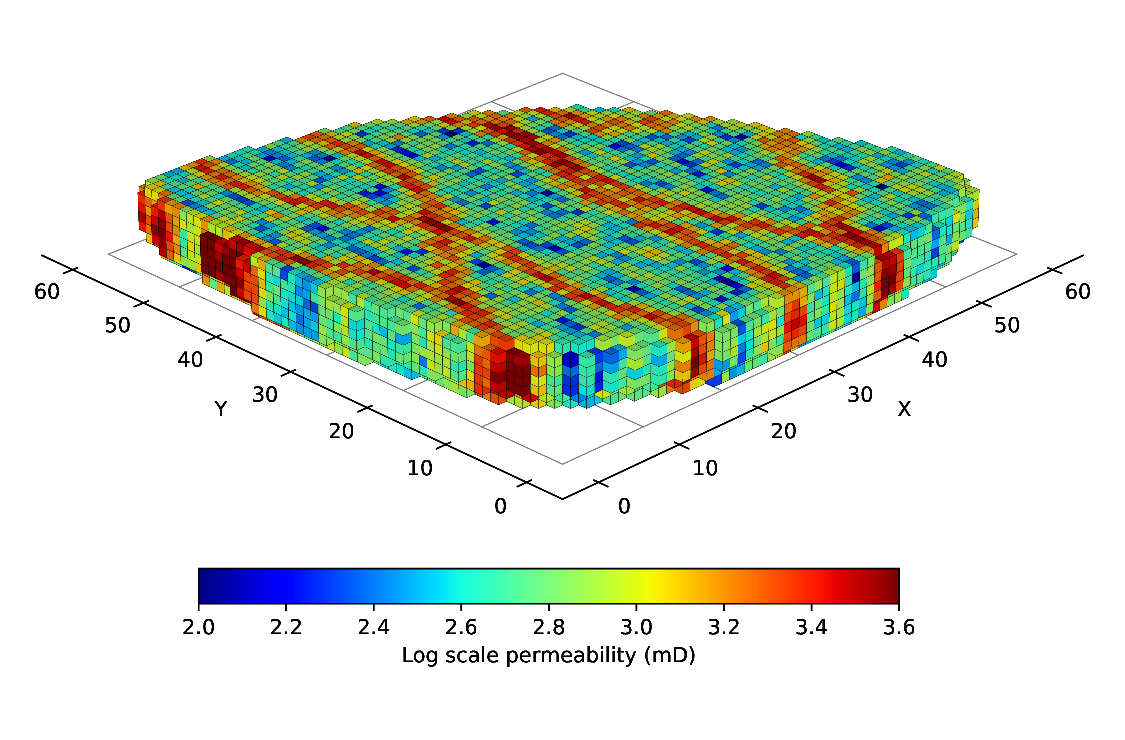
\includegraphics[height=243pt,width=400pt]{images/egg_model_log_3D.eps}
    \caption{3D Egg model}\label{fig:2}
  \end{center}
\end{figure}

\section{Incertezas do Mercado}

A hematita é o mineral de ferro mais importante devido a sua alta
ocorrência em vários tipos de rochas e suas origens diversas.
A composição química deste mineral é Fe$_{2}$O$_{3}$, com uma fração
mássica em ferro de 69,9\% e uma fração mássica em oxigênio de

\section{Redes Neurais}

A hematita é o mineral de ferro mais importante devido a sua alta
ocorrência em vários tipos de rochas e suas origens diversas.
A composição química deste mineral é Fe$_{2}$O$_{3}$, com uma fração
mássica em ferro de 69,9\% e uma fração mássica em oxigênio de

\section{Redes Neurais Convolucionais}

A hematita é o mineral de ferro mais importante devido a sua alta
ocorrência em vários tipos de rochas e suas origens diversas.
A composição química deste mineral é Fe$_{2}$O$_{3}$, com uma fração
mássica em ferro de 69,9\% e uma fração mássica em oxigênio 















